\documentclass[tikz,border=5pt]{standalone}
\usepackage{tikz}
\usepackage{pgfplots}
\usepackage{lmodern}
\pgfplotsset{compat=1.18}

\begin{document}
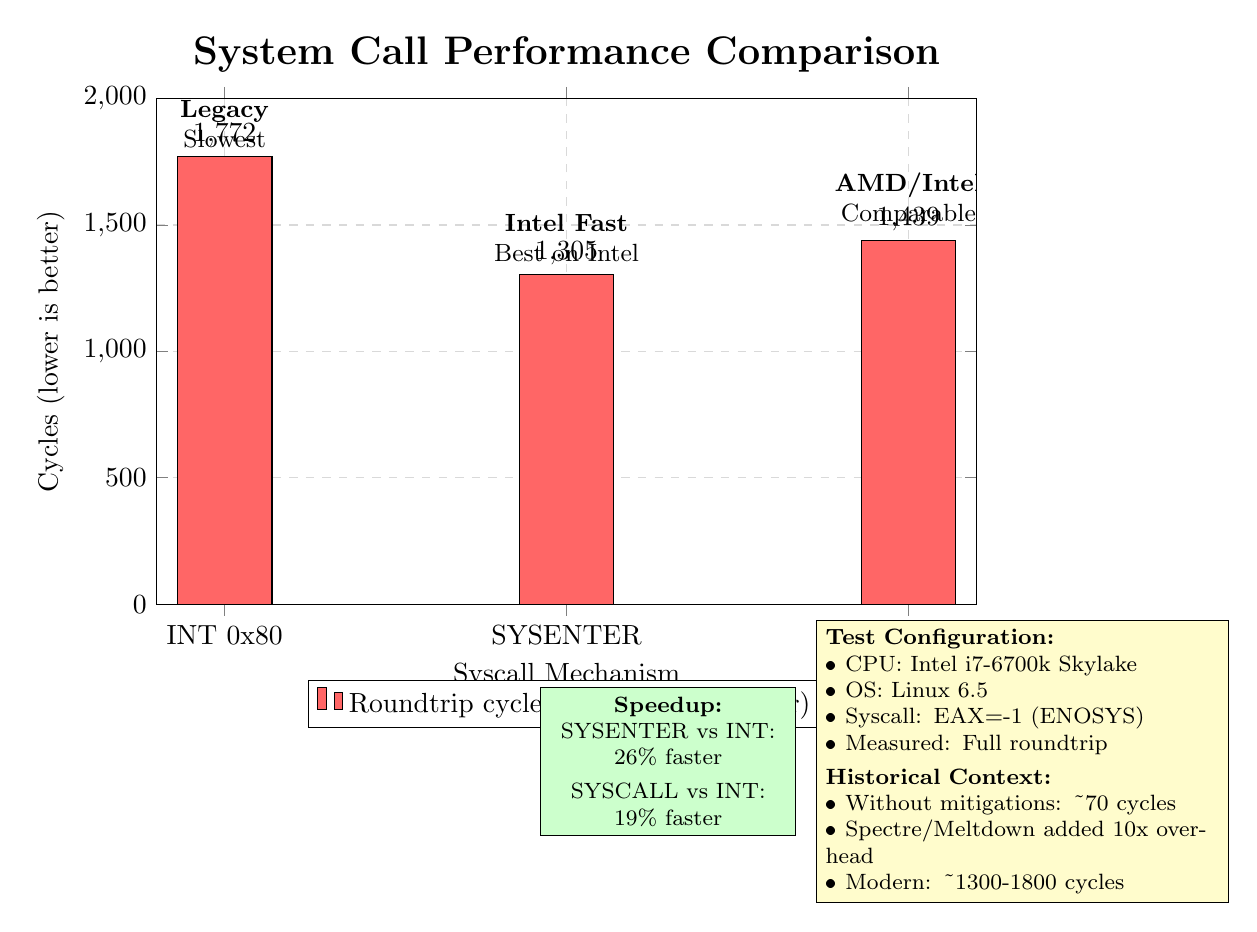
\begin{tikzpicture}
\begin{axis}[
    title={\Large\textbf{System Call Performance Comparison}},
    xlabel={Syscall Mechanism},
    ylabel={Cycles (lower is better)},
    ybar,
    bar width=1.2cm,
    width=12cm,
    height=8cm,
    ymin=0,
    ymax=2000,
    xtick=data,
    symbolic x coords={INT 0x80, SYSENTER, SYSCALL},
    nodes near coords,
    nodes near coords align={vertical},
    legend style={at={(0.5,-0.15)},anchor=north},
    grid=major,
    grid style={dashed,gray!30}
]

% Data from benchmarks (Skylake i7-6700k, Linux 6.5)
\addplot[fill=red!60] coordinates {
    (INT 0x80, 1772)
    (SYSENTER, 1305)
    (SYSCALL, 1439)
};
\legend{Roundtrip cycles (user→kernel→user)}

% Annotations
\node[font=\small,align=center] at (axis cs:INT 0x80,1900) {
    \textbf{Legacy}\\
    Slowest
};
\node[font=\small,align=center] at (axis cs:SYSENTER,1450) {
    \textbf{Intel Fast}\\
    Best on Intel
};
\node[font=\small,align=center] at (axis cs:SYSCALL,1600) {
    \textbf{AMD/Intel}\\
    Comparable
};

\end{axis}

% Additional info box
\node[font=\footnotesize,fill=yellow!20,draw,text width=5cm,align=left] at (11,-2) {
    \textbf{Test Configuration:}\\
    • CPU: Intel i7-6700k Skylake\\
    • OS: Linux 6.5\\
    • Syscall: EAX=-1 (ENOSYS)\\
    • Measured: Full roundtrip\\
    \vspace{0.1cm}
    \textbf{Historical Context:}\\
    • Without mitigations: \textasciitilde70 cycles\\
    • Spectre/Meltdown added 10x overhead\\
    • Modern: \textasciitilde1300-1800 cycles
};

% Speedup annotation
\node[font=\footnotesize,fill=green!20,draw,text width=3cm,align=center] at (6.5,-2) {
    \textbf{Speedup:}\\
    SYSENTER vs INT:\\
    26\% faster\\
    \vspace{0.1cm}
    SYSCALL vs INT:\\
    19\% faster
};

\end{tikzpicture}
\end{document}
